\section{Partial Solution}

The problem \ref{prob:partial} is different from other graph partitioning problems at the objective function. Unlike other problems, our objective function is not even polynomial-time computable (Travelling Salesman Problem). Isaac Vandermeulen, Roderich Groß, Andreas Kolling~\cite{vandermeulen2019balanced} have introduced a clever technique to obtain an approximation solution to the problem. In this section, we introduce a method to approximate the solution of problem \ref{prob:partial} that fills some gaps in the original method.

\subsection{Preliminaries}

Consider the problem of minimizing a function $f: D \to \mathbb{R}$

In many scenarios, it is hard to find an optimal, or it is even also hard to compute the value of $f$.
The method below was inspired from the work of Isaac Vandermeulen, Roderich Groß, Andreas Kolling~\cite{vandermeulen2019balanced}.

For a domain $X \subseteq D$ of the minimization problem,  let $f_1: X \to \mathbb{R}$ be the proxy function such that
\[
    (1): f(x) = c(f_1(x)) + v(x) \text{ } \forall x \in x
\]


Where $c$ is a monotonically increasing function and $v: X \to \mathbb{R}$ is function on $X$.

Let $x^*$ and $x^*_1$ be the optimal values for $f$ and $f_1$ in the domain $X \subseteq D$.
Let $t_{\max} = \max_{x \in X} v(x)$ and $t_{\min} = \min_{x \in X} v(x)$ be the maximum value and minimum value of $v$ over the domain $X$. 

\begin{figure}[h!]
\centering
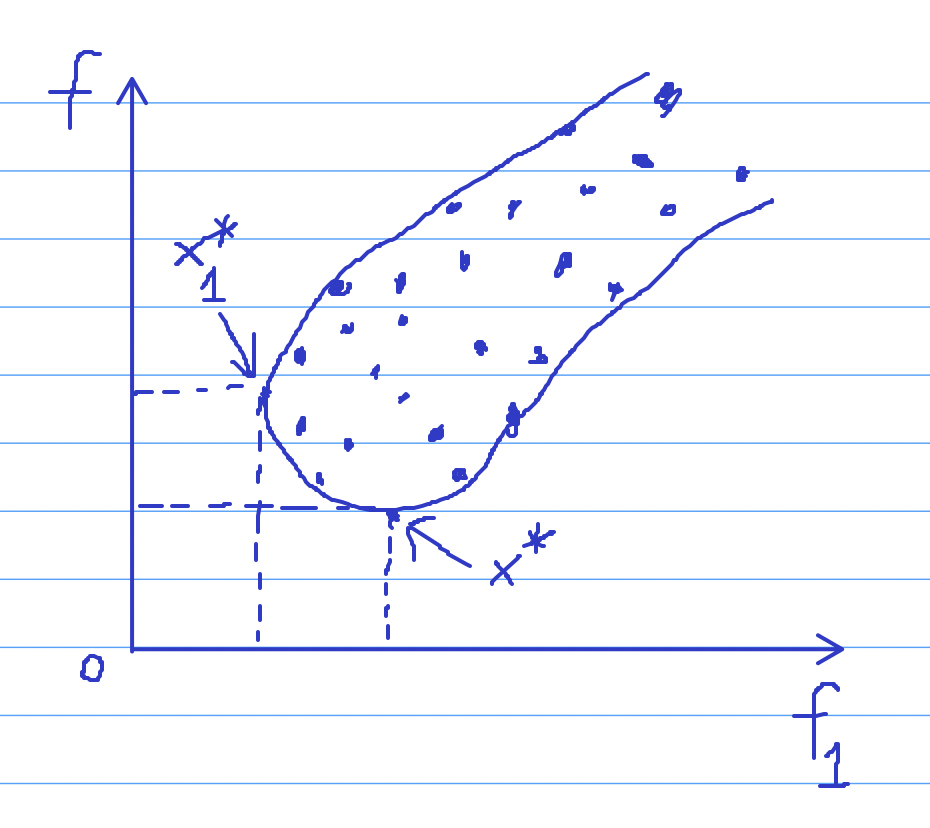
\includegraphics[width=0.8\textwidth]{assets/f1_approximation.png}
\caption{$f_1$ approximation}
\label{fig:f1_approximation}
\end{figure}

\begin{theorem}[$f_1$ approximation]
\[
    f(x^*_1) \leq f(x^*) + (t_{\max} - t_{\min})
\]
\label{theo:f1_approximation}
\end{theorem}

The theorem \ref{theo:f1_approximation} provides us a guarantee on how good the solution of $f_1$ in minimizing $f$. By finding an appropriate proxy function $f_1$, we can find an approximation on $f$.

\subsection{Proxy Function}

In \cite{vandermeulen2019balanced}, in order to minimize the maximum tour cost, the authors introduced a proxy function $f_1$ to be the maximum of average tour cost of the $K$ tours and a local search algorithm to find a local optimal. However, the function does only capture the maximum-length tour over the $K$ tours that does not allow the local search to enhance to total tour cost and potentially traps the algorithm in a bad region in the search space. We introduce three proxy function as follow:

Given $K$ partitions of the graph $G_P$, each partition is a disjoint subset of nodes in $G_P$ (a subset of POIs). Denote $C_m^{(k)}$ to be the minimum tour cost of the $k$-th partition (TSP tour cost). Our objective function is to find a partitioning of $K$ partition such that the objective is minimized:

\[
f(.) = \max\{C_m^{(k)}\}_{k=1}^{K} = ||C_m||_\infty
\]

\subsubsection{Maximum of Average Tour Cost and Sum of Average Tour Cost}

In \cite{vandermeulen2019balanced}, denote $C_a^{(k)}$ to be the average tour cost if the $k$-th partition where the average tour cost in a graph is defined as expected value of a tour when the node ordering is chosen at uniformly random order all possible ordering. Let $V_P^{(k)}$ be the set of POIs in the $k$-th partition. $C_a^{(k)}$ can be calculated by:

\[
C_a^{(k)} = \frac{1}{|V_P^{(k)}| - 1} \sum_{v_i \in V_P^{(k)}} \sum_{v_j \in V_P^{(k)} \backslash \{v_i\}} c_P((v_i, v_j))
\]

Let $A_P^{(k)}$ be the adjacency of the sub-graph induced by $V_P^{(k)}$ with zeros on diagonal, then $C_a^{(k)}$ can also be calculated as the sum of all entries divided by $|V_P^{(k)}| - 1$.

\[
C_a^{(k)} = \frac{\mathds{1}^T A_P^{(k)} \mathds{1}}{|V_P^{(k)}| - 1}
\]

The author used maximum of average tour cost:

\[
f_1(.) = O_0(.) = \max\{C_a^{(k)}\}_{k=1}^{K} = ||C_a||_\infty
\]

Based on the same concept of average tour cost, we introduce the sum of average tour cost:

\[
f_1(.) = O_8(.) = \sum_{k=1}^{K} C_a^{(k)} = ||C_a||_1
\]

Another trivial extension is to interpolate $O_0(.)$ and $O_8(.)$:

\[
f_1(.) = O_9(.) = \alpha ||C_a||_\infty + \beta ||C_a||_1
\]

for $\alpha + \beta = 1$ and $\alpha, \beta \geq 0$
Or, 

\[
f_1(.) = O_{10}(.) = \frac{1}{K}\sum_{k=1}^{K}\log C_a^{(k)}
\]

Given a set of partitioning where $O_8(.)$ have the same objective value, $O_{10}(.)$ will find the most balanced partitioning \footnote{$O_{10}(.)$ converges at the middle of the simplex}. Given a set of partitions where $O_0(.)$ have the same objective value, $O_{10}(.)$ will find the least cost partitioning \footnote{zero all other partitions except the maximum one}. \footnote{hand-wavy argument}

By log concavity, $O_{10}(.)$ lies somewhere between $O_0(.)$ and $O_8(.)$

\[
\frac{1}{K} \log \max \{C_a^{(k)}\}_{k=1}^{K} \leq \frac{1}{K}\sum_{k=1}^{K}\log C_a^{(k)} \leq - \log K + \log \sum_{k=1}^{K} C_a^{(k)}
\]

Furthermore, this function encourage partitions being more balanced \footnote{A similar proof can be found in Appendix}


\subsubsection{Other Handcrafted Tour Cost}

Let $A$ be the adjacency matrix of $G_P$ defined by:

\[
A_{ij} = c_P((v_i, v_j))
\]

where $c_P((v_i, v_i)) = 0$ $\forall v_i \in V_P$ (diagonal entries are all zero).

Let $x^{(k)} \in \{0, 1\}^{|V_P|}$ be an indicator vector of $k$-th partition.

\[
x^{(k)}_i = \{
        \begin{array}{ll}
            1 \;\;\;\; \text{if $i \in V_P^{(k)}$}\\
            0 \;\;\;\; \text{otherwise}
        \end{array}
\]

Since, $K$ partitions are disjoint, we have an orthogonal constraint on $x^{(k)}$ such that $\forall k_1 \neq k_2$, $x^{(k_1)T} x^{(k_2)} = 0$

For the $k$-partition, the quadratic form $x^{(k)T} A x^{(k)}$ equals the sum of all entries in the sub-graph adjacency matrix $A_P^{(k)}$ induced by $V_P^{(k)}$. We have:

\[
C_a^{(k)} = \frac{x^{(k)T} A x^{(k)}}{|V_P^{(k)}| - 1} = \frac{x^{(k)T} A x^{(k)}}{x^{(k)T} x^{(k)} - 1} 
\]

We use the proxy function defined by:

\[
f_1(.) = O_1(.) = \sum_{k=1}^{K} \frac{x^{(k)T} A x^{(k)}}{x^{(k)T} x^{(k)}}
\]

At this stage, we relax our 0-1 constraint to the indicator vector. Minimizing $O_1(.)$ with respect to the orthogonal constraint yields the $K$ smallest eigenvalues. The minimal is at $K$ corresponding eigenvectors.

The objective $O_1(.)$ is very close to the sum of average tour cost function. However, we are finding the partition such that the maximum tour cost should be minimized. We introduce a more complex proxy function as follow:

\[
f_1(.) = O_7(.) = 
\sum_{k=1}^{K} \frac{x^{(k)T} (A - \alpha D) x^{(k)}}{x^{(k)T} x^{(k)} + \beta |V_P|}
=
\sum_{k=1}^{K} \frac{\sum_{i \in V_k} \sum_{j \in V_k} A_{ij}}{|V_P^{(k)}| + \beta |V_P|} - \alpha \frac{\sum_{i \in V_k} D_{ii}}{|V_P^{(k)}| + \beta |V_P|}
\]

where $\alpha$ and $\beta$ are two careful chosen non-negative parameters and $D$ is the degree matrix of $A$

Constant $\beta$ makes the partitions more balanced. Let $\alpha = 0$, consider a graph that all edges have unit length. A positive constant $\beta$ makes the unique minimum partition to be the balanced one. \footnote{Detailed analysis in Appendix}

Constant $\alpha$ is intended to encourage large degree nodes to join the small partitions.

If $\alpha = 0$ and $\beta = 0$, we obtain $O_8(.)$. If $\alpha \in \{0, 1\}$ and $\beta \to +\infty$, we obtain the objective function of MAX-CUT problem.

In the experiment, we have chosen $\alpha = 0$ and $\beta = 1$.

Instead of the orthogonal constraint, we imposed a pair of constraints for the indicator vectors. This can be thought as representing each entry by the probability of the corresponding POIs belong to

\[
x^{(k)} \succeq 0 \text{ and } \sum_{k=1}^{K} x^{(k)} = \mathds{1}
\]

The pair of constraints  makes $x^{(k)}$ as a soft indicator. In the experiment, we changed the second constraint to be inequality.

\[
x^{(k)} \succeq 0 \text{ and } \sum_{k=1}^{K} x^{(k)} \succeq \mathds{1}
\]

Finally, the partition for each POI is taken as:

\[
k_i = \argmax_k \{x^{(k)}_i\}_{k=1}^{K} 
\]

In the experiment, most of the time, entries of $x^{(k)}$ always converge to either 0 or 1.

In the experiment, minimizing $O_0(.)$ and $O_7(.)$ tends to reduce the maximum tour cost while minimizing $O_1(.)$ and $O_8(.)$ tends to reduce the sum of tour cost.

\begin{figure}[h!]
\centering
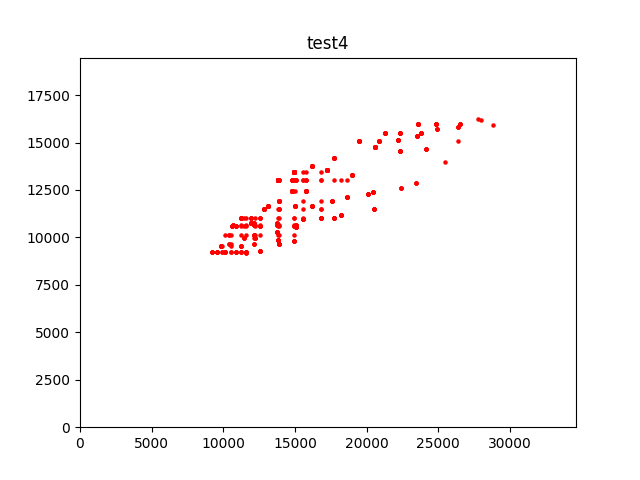
\includegraphics[width=0.8\textwidth]{assets/test0max.png}
\caption{maximum of tour cost over $O_0(.)$ of all 5-partitions in a 15 nodes network}
\label{fig:test0max}
\end{figure}

\begin{figure}[h!]
\centering
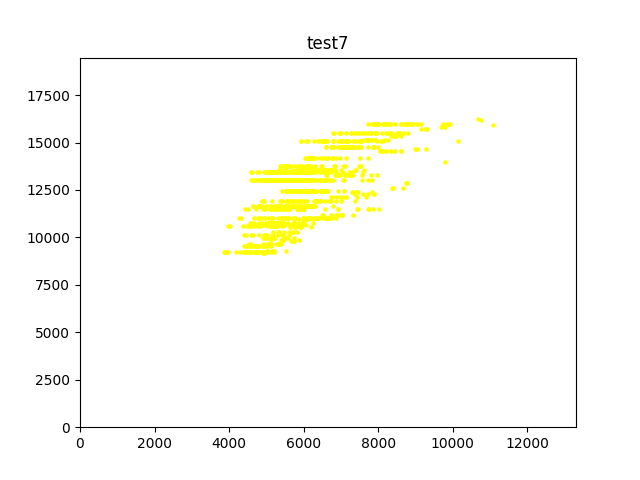
\includegraphics[width=0.8\textwidth]{assets/test7max.png}
\caption{maximum of tour cost over $O_7(.)$ of all 5-partitions in a 15 nodes network}
\label{fig:test7max}
\end{figure}

\begin{figure}[h!]
\centering
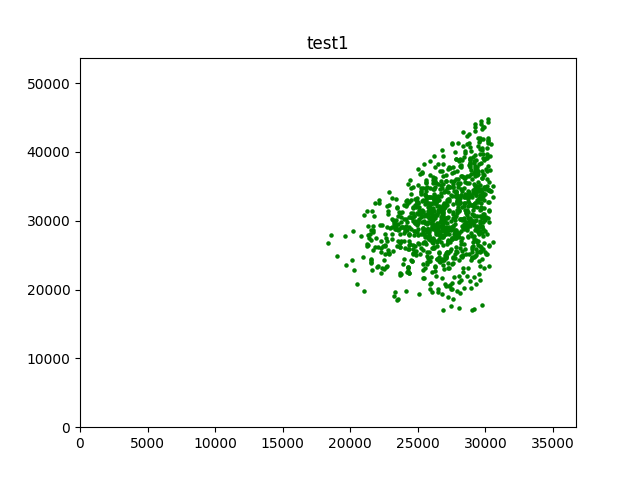
\includegraphics[width=0.8\textwidth]{assets/test1sum.png}
\caption{sum of tour cost over $O_1(.)$ of all 5-partitions in a 15 nodes network}
\label{fig:test1sum}
\end{figure}

\begin{figure}[h!]
\centering
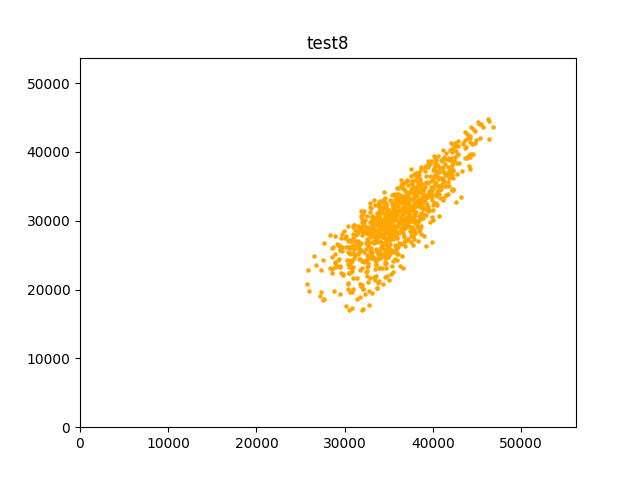
\includegraphics[width=0.8\textwidth]{assets/test8sum.png}
\caption{sum of tour cost over $O_8(.)$ of all 5-partitions in a 15 nodes network}
\label{fig:test8sum}
\end{figure}

\subsection{Optimizing Proxy Function}

For $O_1(.)$ and $O_8(.)$, we use local search to obtain the local optimal partition. From the existing work, we use two operations defining neighbour in the search space: (\textbf{1. Transfer}) A POI is transferred from one partition to another partition. (\textbf{2. Swap}) A pair of POIs from two different partitions are swapped.

On the other hand, $O_1(.)$ can be solved using standard eigen-solver and $O_7(.)$ can be solved using standard constrained optimization techniques.